\section{Cross-Vendor Replication}

\subsection{Method}

We designed prompts for all three strategies described by Leyva-Vázquez
and Smarandache (see Appendix A for full prompts):

\begin{itemize}
\tightlist
\item
  \textbf{S1 (Neutrosophic)}: Independent T, I, F on {[}0,1{]},
  explicitly stated as not constrained to sum to 1.0
\item
  \textbf{S2 (Probabilistic)}: T + I + F constrained to 1.0
\item
  \textbf{S3 (Entropy-Derived)}: Binary P(yes)/P(no), indeterminacy
  derived from Shannon entropy: H = -(p$\cdot$log$_{2}$p + (1-p)$\cdot$log$_{2}$(1-p)). Note:
  since T=P\_yes and F=P\_no with T+F=1.0 by construction, S3 Sum = 1.0
  + H, meaning S3 produces hyper-truth by mathematical construction
  whenever P\_yes is not exactly 0 or 1. S3 hyper-truth rates are
  therefore not directly comparable to S1 and are not used in our
  analysis
\end{itemize}

We evaluated five models from five vendors via OpenRouter's
OpenAI-compatible API:

\begin{longtable}[]{@{}lll@{}}
\toprule\noalign{}
Model & Provider & Parameters \\
\midrule\noalign{}
\endhead
\bottomrule\noalign{}
\endlastfoot
Claude Sonnet 4.6 & Anthropic & Undisclosed \\
Llama 4 Maverick & Meta & Undisclosed \\
DeepSeek V3 & DeepSeek & 671B MoE \\
Qwen3-235B & Alibaba & 235B MoE \\
Mistral Medium 3.1 & Mistral & Undisclosed \\
\end{longtable}

Each cell was evaluated 5 times (temperature=0.7), yielding 375
evaluations (5 models × 5 phenomena × 3 strategies × 5 reps). Of these,
373 produced valid JSON parses; 2 responses were garbled or truncated (1
DeepSeek, 1 Llama) and are excluded from analysis. All data, code, and
prompts are published in the repository.

\textbf{Important caveat}: Because the original prompts were not
published, we designed our prompts from the strategy descriptions in the
paper. We cannot claim direct replication, which is a parallel
experiment with independently constructed prompts. The S2 control
(below) provides evidence that our prompt framing is not radically
different from the original.

\subsection{Results}

\textbf{S2 constraint validation.} Under probabilistic constraint (S2),
all 125 evaluations across all models and phenomena produced Sum = 1.000
± 0.000, with 0\% hyper-truth. This matches the original study exactly
and provides evidence that our prompt construction is compatible with
theirs: the constraint mechanism behaves identically.

\textbf{S1 hyper-truth is cross-vendor and amplified.} Under
unconstrained neutrosophic evaluation (S1):

\begin{longtable}[]{@{}llll@{}}
\toprule\noalign{}
Model & Hyper\% & Mean Sum & CV(Sum) \\
\midrule\noalign{}
\endhead
\bottomrule\noalign{}
\endlastfoot
Claude Sonnet 4.6 & 100\% & 1.810 & 0.110 \\
DeepSeek V3 & 100\% & 1.475 & 0.161 \\
Qwen3-235B & 80\% & 1.464 & 0.242 \\
Llama 4 Maverick & 76\% & 1.348 & 0.230 \\
Mistral Medium 3.1 & 64\% & 1.312 & 0.281 \\
\end{longtable}

Overall S1 hyper-truth: 84\% (104/124 valid cells; 1 garbled response
excluded), compared to the original study's 35\% (7/20 cells).
Hyper-truth is not an OpenAI artifact as it emerges across all five
vendor families.

\textbf{Phenomenon-level comparison with original:}

\begin{longtable}[]{@{}llll@{}}
\toprule\noalign{}
Phenomenon & Original Sum & Ours (S1) & Delta \\
\midrule\noalign{}
\endhead
\bottomrule\noalign{}
\endlastfoot
Paradox (Logical) & 1.500 & 1.480 & -0.020 \\
Ignorance (Epistemic) & 1.125 & 1.526 & +0.401 \\
Vagueness (Fuzzy) & 1.125 & 1.382 & +0.257 \\
Contradiction (Ethical) & 1.475 & 1.690 & +0.215 \\
Contingency (Future) & 1.000 & 1.325 & +0.325 \\
\end{longtable}

Ethical contradiction achieves 100\% hyper-truth across all models in
our data, confirming the original study's finding that moral conflict is
the strongest driver of hyper-truth.

\subsection{Three Philosophical Positions on Paradox}

The liar's paradox (``This sentence is false'') reveals three distinct
interpretations of T/I/F. Three of five models (Claude, DeepSeek, Llama)
show zero intra-model variance across all 5 repetitions. Mistral is
near-consistent (4/5 reps identical, 1 outlier). Qwen shows position
instability, adopting different positions across reps.

\textbf{Position 1: Saturation} (Claude, 5/5 reps): T=0.5, I=1.0, F=0.5,
Sum=2.0. The paradox is simultaneously half-true, half-false, and
maximally indeterminate. All three dimensions are active independently.

\textbf{Position 2: Balanced Conflict} (DeepSeek, 5/5 reps): T=0.5,
I=0.5, F=0.5, Sum=1.5. Equal truth and falsity with moderate
indeterminacy. The paradox creates contradiction but not maximal
uncertainty.

\textbf{Position 3: Absorption} (Llama 5/5, Mistral 4/5): T=0.0, I=1.0,
F=0.0, Sum=1.0. Indeterminacy absorbs truth value entirely. The paradox
is treated as having no truth value, effectively the classical logic
response of rejecting the statement as malformed.

Qwen alternates between Positions 1 and 3, suggesting the model has not
converged on a stable interpretation of the paradox.

\begin{figure}
\centering
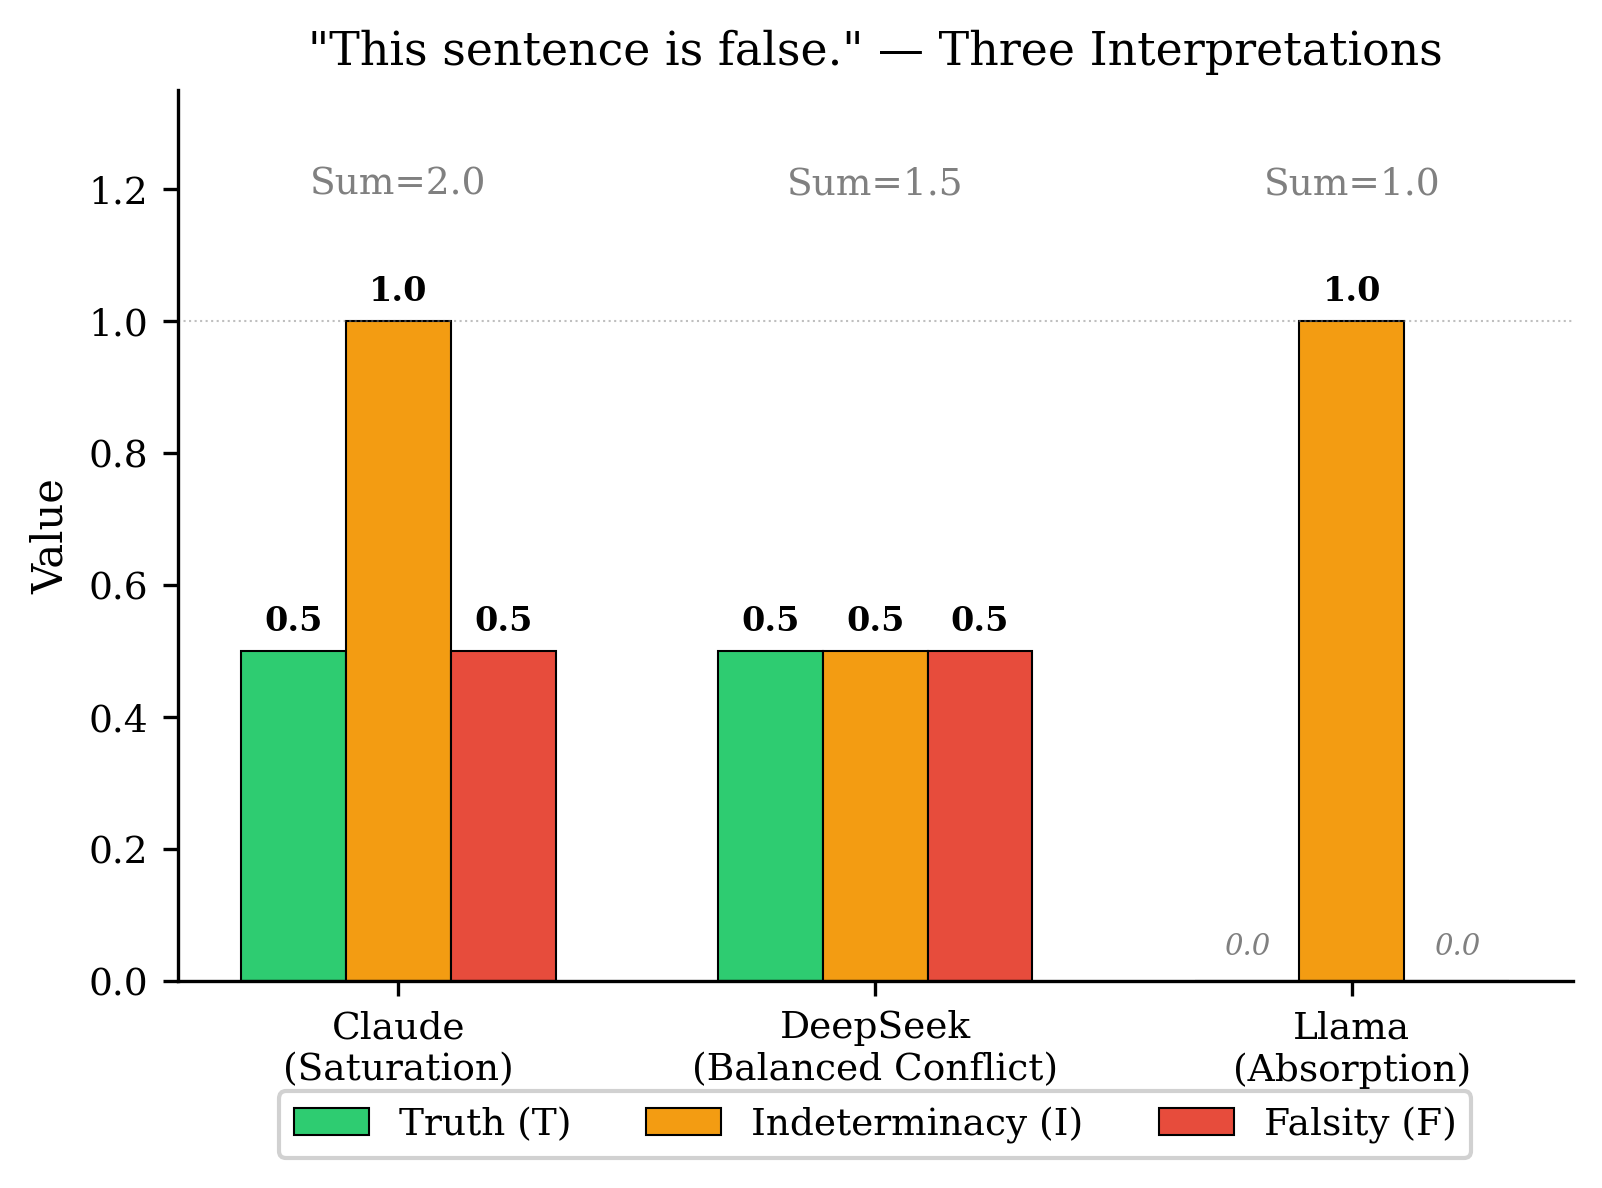
\includegraphics{fig_paradox_positions.png}
\caption{Figure 1: Three philosophical positions on the liar's paradox}
\end{figure}

\emph{Figure 1: T/I/F values for ``This sentence is false'' across three
models exhibiting distinct interpretations. Absorption (Llama) collapses
T and F to zero, leaving only I --- the same scalar output as ignorance
and contingency.}

These positions are invisible to any metric based on Sum alone. The
original study, which reported only sum-based analysis, could not have
detected them.

Critically, the Absorption position (Position 3) creates a problem for
neutrosophic logic itself: models predominantly adopting this position
produce near-identical T/I/F scalars for paradox, ignorance, and
contingency, which are three fundamentally different types of
uncertainty. The scalar representation collapses exactly the
distinctions neutrosophic logic was designed to preserve.
